%%%%%%%%%%%%%%%%%%%%%%%%%%%%%%%%%%%%%%%%%%%%%%%%%%%%%%%%%%%%%%%%%%%%%%%
% Based on IEEE the conference template available                     %
% at https://www.ieee.org/conferences/publishing/templates.html       %
% Adapted for the Data Science Lab course at Politecnico di Torino    %
% by Giuseppe Attanasio, Flavio Giobergia                             %
% 2020, DataBase and Data Mining Group                                %
%%%%%%%%%%%%%%%%%%%%%%%%%%%%%%%%%%%%%%%%%%%%%%%%%%%%%%%%%%%%%%%%%%%%%%%

\documentclass[conference]{IEEEtran}
\usepackage[skip=0.5\baselineskip]{caption}
\usepackage{cite}
\usepackage{amsmath,amssymb,amsfonts}
\usepackage{algorithmic}
\usepackage{graphicx}
\usepackage{textcomp}
\usepackage{xcolor}
\usepackage{hyperref}
\usepackage{multirow}


\begin{document}

\title{Deep Learning for Audio Classification:\\ 
An Overview and Analysis }

\author{\IEEEauthorblockN{Gaetano Salvatore Falco}
\IEEEauthorblockA{\textit{Politecnico di Torino} \\
Student id: s280209 \\
\href{mailto:gaetanosalvatore.falco@studenti.polito.it}{gaetanosalvatore.falco@studenti.polito.it}
%gaetanosalvatore.falco@studenti.polito.it} 
 }
\and
\IEEEauthorblockN{ Kuerxi Gulisidan}
\IEEEauthorblockA{\textit{Politecnico di Torino} \\
Student id: s304915 \\
\href{mailto:kuerxi.gulisidan@studenti.polito.it}{kuerxi.gulisidan@studenti.polito.it}
}
}

\maketitle
\begin{abstract}
In this report, we propose a deep learning-based method for classifying audio recordings based on the intent expressed in them. The proposed approach utilizes a Depthwise Separable Convolutional Neural Network (DS-CNN) to predict both the action request and the object affected by the action. Our method begins with standardizing and preprocessing the input data, which is crucial for achieving high accuracy in the model. We then build a CNN model to classify intents in the evaluation set. The performance of our model is evaluated using accuracy, and the results demonstrate the effectiveness of the proposed approach.\\
All code is publicly available at: \url{https://github.com/chowned/Audio-recognition-for-IOT}

\end{abstract}

\section{Problem overview}
In recent years, there has been a growing interest in developing methods for automatically classifying audio recordings based on the intent expressed in them. The ability to accurately understand and interpret human speech is crucial for a wide range of applications, including speech recognition, natural language understanding, and human-computer interaction.
For this project, we will work on an intent detection problem given an input audio sample. The goal of this project is to predict both the requested action and the object that is affected by the action.\\
The dataset is divided into the following parts:
\begin{itemize}
 \item 	\textbf{audio}: containing 11309 WAV format audio files recorded by 97 speakers
 \item 	\textbf{development.csv}: a comma-separated values file containing the records from the development set.
 \item 	 \textbf{evaluation.csv}: a comma-separated values file containing the records corresponding to the evaluation set.
\end{itemize}
This problem is made even more difficult by the variability in the way that different speakers express the same intent.

When reviewing the development.csv file, we can see that it contains 10 columns and 9854 rows, leveraged to obtain the labels required for training and validating models. The evaluation set contains 8 columns and has 1454 rows, lacking the action and object columns that have to be predicted.\\

\vspace{20mm}

The provided dataset is characterized by the following columns:


\begin{center}
\begin{tabular}{ |c| } 

 \hline
 Id   \\ 
  \hline
 path  \\
  \hline
 speakerID\\
  \hline
 \textbf{action}\\
  \hline
 \textbf{object}   \\
  \hline
 self-reported fluency level  \\ 
 \hline
 first language spoken \\
 \hline
 gender\\ 
 \hline
 ageRange   \\ 
 \hline
 current language used for work/school   \\ 
 \hline

\end{tabular}
\end{center}

\vspace{5mm}

\section{Proposed approach}
\vspace{5mm}
\subsection{Automatic Audio length finder with given threshold}
After some data exploration, we found out that the provided dataset is composed of audio files of different lengths, according to Fig.1.

\begin{figure}[h]
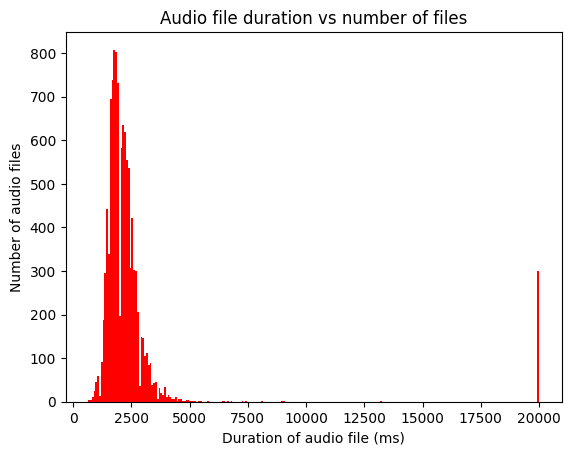
\includegraphics[width=9cm]{audio_file_graph.png}
\caption{Audio file duration}
\label{fig1}
\end{figure}

As we have to build a model and specify the input shape, we found it necessary to standardize our input data. We developed the "find\_duration" function to accomplish this task and, provided a threshold of 90\%, it returns the audio length that is able to incorporate such a percentage. This length was saved as a variable in seconds and used to standardize the length of the entire dataset through padding.\\
While the audio length in the dataset was spread as a normal distribution with outliers, we chose to use the "find\_duration" function instead of calculating the mean and standard deviation as it is not dependent on the initial distribution.



\subsection{Data Preprocessing}

In this section, we describe the preprocessing steps taken on the audio files to normalize and standardize them for the model. The goal of this preprocessing is to ensure that all audio files share a common ground in terms of sampling rate and duration.
\begin{itemize}
\item 	\textbf{Sampling rate}: 8.000, this gives us a good balance between audio quality and prediction time.
\item 	\textbf{Duration}: 4s, this is automatically found by the "find\_duration" function
\end{itemize}
We use the librosa library to trim the audio files, remove silence and change the sampling rate if it is different by calling the "process\_file" function according to these steps:
\begin{itemize}
\item 	\textbf{Label building}: as we have to predict both the object and the action, we use this information to build the corresponding label for each audio file.
\item 	\textbf{Audio trim}: We remove silence from the audio files. This could be a huge problem if we start by cutting the length at 4s and our speaker starts to talk after 3 seconds.
\item 	\textbf{Resample and padding}: as there are different sampling rates in the provided dataset, we make sure the output sampling rate is 8.000 and, if the input audio file after the trim operation is less than 4s, we increase its duration by using padding and make it compliant with out choices.
\item 	\textbf{Storing the audio files}: as we want to fine-tune the hyperparameters of our model, applying these steps at each run is a huge workload. We then decided to save both the development dataset and the evaluation dataset into two folders, which will be called by the model for the prediction.
\end{itemize}
We eventually proceed to use the "preprocess" function on the training and test set, which will perform these actions:
\begin{itemize}
\item 	\textbf{Input audio to mono channel}: we decide to convert all of our audio files to a single channel, as this is more than enough to store the necessary information.
\item 	\textbf{STFT}: we apply a short-time Fourier transform to convert the audio files from the time domain to the frequency domain, and then we compute the spectrogram by taking the absolute value of the STFT result.
\item 	\textbf{MFCCs}: we have chosen an audio representation based on extracting the features as Mel-frequency cepstral coefficients. This allows us to carry the most valuable information while also being able to use convolutional layers in our model.
\end{itemize}
In the following figures, an example of the audio stream as it is passed to the model. In figure 2 there is an example for the audio with label "activate music" while in figure 3 an example for the audio with label "increase heat".
\\These examples also allows us to show the results of the padding function, and to better show that no information is carried to the model that can focus only on the part that carries the information.

\begin{figure}[h]
\includegraphics[width=9cm]{activatemusic.png}
\caption{"1-activatemusic"}
\label{fig1}
\end{figure}

\begin{figure}[h]
\includegraphics[width=9cm]{increaseheat.png}
\caption{"6-increaseheat"}
\label{fig1}
\end{figure}


\subsection{Model selection}
Our approach to audio classification is mainly based on the researches done by Palanisamy et al. [1] and Peter Mølgaard Sørensen et al.[2]. One proposed a method of using pre-trained convolutional neural networks (CNNs) for audio classification, by using transfer learning on the weights instead of random initialization. Another one proposed a depthwise separable convolutional neural network for keyword spotting. The approach has been proven to achieve state-of-the-art performance by utilizing the Mel-frequency cepstral coefficients (MFCCs) technique, which is implemented in the provided code for data preprocessing. This method allows us to extract relevant features from the audio data and uses them to train a CNN model that is fine-tuned for the task of audio classification. Overall, this approach is a promising way to achieve high accuracy in audio classification tasks.\\


\subsection{Hyperparameters tuning}
The training of the Depthwise Separable Convolutional Neural Network (DS-CNN) was carried out using a learning rate of 0.01, a batch size of 32, and 512 output filters in the convolution. Due to limited resources, the number of filters was reduced by multiplying it with an alpha of 0.125 to speed up the training process. The following hyperparameters were optimized to obtain the best combination:
\begin{itemize}
\item 	\textbf{Frame length}: set to 0.064 seconds
\item 	\textbf{Frame step}: set to 0.064 seconds
\item 	\textbf{Lower frequency}: set to 20 Hz
\item 	\textbf{Higher frequency}: set to sampling rate/2 = 4,000 Hz
\end{itemize}

To monitor the training and evaluate the results, TensorBoard was used along with different callbacks.The rest of the network is initialized with Xavier initialization, and all parameters are updated during training with the Adam optimizer while a linear decay was set for the learning rate. The training was early stopped when the accuracy on the training set reached 100\%.

\vspace{5mm}
\section{Results}
We tested out model with different batch size and alpha values and the results are shown in the table below. Incremented alpha value has shown to give better results, at the expense of being more time consuming.




\vspace{5mm}

\begin{table}[h]
\centering
\begin{tabular}{ |l|l|l| }
\hline
\multicolumn{3}{ |c| }{Hyper-parameters Grid Search} \\
\hline \hline
Alpha & Batch size  & Test Accuracy \\ \hline\hline
\multirow{5}{*}{0.125} & 64 & 0.885 \\
 & 32 & 0.889 \\
 & 16 & 0.920 \\
 & 8 & 0.907 \\
 & 4 & 0.889 \\ \hline
 \multirow{5}{*}{1} & 64 & 0.940 \\
 & 32 &\textbf{0.959} \\
 & 16 & 0.951 \\
 & 8 & 0.945 \\
 & 4 & 0.956 \\ 

\hline
\end{tabular}
\caption{}
\end{table}

\vspace{5mm}

\section{Discussion}
We hope that this report sparks additional research in the field of audio classification and highlights the potential of a small Convolutional Neural Network (CNN) to achieve high performance. Despite the limited scope of our experiments, the results demonstrate that a CNN with proper hyperparameter tuning is suitable for IoT devices with limited computational resources. We believe that further exploration and optimization of this approach can lead to even better results in the future.

\vspace{5mm}
%\bibliography{bibliography}
\begin{thebibliography}{00}
\bibitem{b1} Kamalesh Palanisamy, Dipika Singhania, Angela Yao, "Rethinking CNN Models for Audio Classification" in arXiv 2020  (\url{https://arxiv.org/pdf/2007.11154.pdf})

\bibitem{b2} Sørensen, P.M., Epp, B. \& May, T. "A depthwise separable convolutional neural network for keyword spotting on an embedded system." J AUDIO SPEECH MUSIC PROC. 2020, 10 (2020). (\url{https://doi.org/10.1186/s13636-020-00176-2})

\bibitem{b3} Mingwen Dong, "Convolutional Neural Network Achieves Human-level Accuracy in Music Genre Classification" in arXiv 2018  (\url{https://arxiv.org/pdf/1802.09697.pdf})

\bibitem{b4} Pete Warden, "Speech Commands: A Dataset for Limited-Vocabulary Speech Recognition" in arXiv 2018 (\url{https://arxiv.org/pdf/1804.03209v1.pdf})

%\bibliographystyle{ieeetr}  [1] PAPER 1 -> https://arxiv.org/pdf/2007.11154.pdf
\end{thebibliography}

\end{document}



